documentclass[tikz,border=5pt]{standalone}
\usepackage{amsmath}
\usetikzlibrary{arrows.meta}

\tikzset{
    >=Latex,
    every label/.style={inner sep=0, font=\scriptsize},
    every node/.style={align=center},
}

\begin{document}
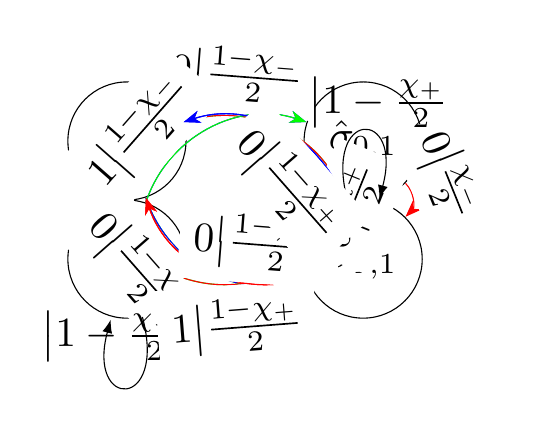
\begin{tikzpicture}[scale=1.5, transform shape]
    \node[circle,draw] (q00) at (-1, 0) {$\hat{\sigma}_{0,0}$};
    \node[circle,draw] (q01) at (1, 0) {$\hat{\sigma}_{0,1}$};
    \node[circle,draw] (q10) at (-1,-1) {$\hat{\sigma}_{1,0}$};
    \node[circle,draw] (q11) at (1, -1) {$\hat{\sigma}_{1,1}$};
    \path [-{Stealth[length=6pt]}]
        (q00) edge [bend left=45,draw=green] node [pos=0.25,above,sloped,fill=white] {$0\big|\frac{\chi_{-}}{2}$} (q11)
        (q00) edge [bend right=45,draw=green] node [pos=0.25,below,sloped,fill=white] {$0\big|\frac{\chi_{+}}{2}$} (q11)
        (q00) edge [bend left=45,draw=red] node [pos=0.25,above,sloped,fill=white] {$0\big|\frac{1-\chi_{-}}{2}$} (q11)
        (q00) edge [bend right=45,draw=blue] node [pos=0.25,below,sloped,fill=white] {$0\big|\frac{1-\chi_{+}}{2}$} (q11)
        (q01) edge [bend left=45,draw=red] node [pos=0.25,above,sloped,fill=white] {$0\big|\frac{\chi_{-}}{2}$} (q11)
        (q01) edge [bend right=45,draw=blue] node [pos=0.25,below,sloped,fill=white] {$0\big|\frac{\chi_{+}}{2}$} (q11)
        (q10) edge [bend left=45,draw=blue] node [pos=0.25,above,sloped,fill=white] {$1\big|\frac{\chi_{-}}{2}$} (q01)
        (q10) edge [bend right=45,draw=green] node [pos=0.25,below,sloped,fill=white] {$1\big|\frac{\chi_{+}}{2}$} (q01)
        (q10) edge [loop below] node [pos=0.7,above] {$\big|1-\frac{\chi_{-}}{2}$} (q10)
        (q10) edge [bend left=45,draw=green] node [pos=0.25,above,sloped,fill=white] {$1\big|\frac{1-\chi_{-}}{2}$} (q01)
        (q10) edge [bend right=45,draw=red] node [pos=0.25,below,sloped,fill=white] {$1\big|\frac{1-\chi_{+}}{2}$} (q01)
        (q11) edge [loop above] node [pos=0.7,above] {$\big|1-\frac{\chi_{+}}{2}$} (q11)
        (q11) edge [bend left=45,draw=red] node [pos=0.25,above,sloped,fill=white] {$0\big|\frac{\chi_{-}}{2}$} (q00)
        (q11) edge [bend right=45,draw=blue] node [pos=0.25,below,sloped,fill=white] {$0\big|\frac{\chi_{+}}{2}$} (q00)
        (q11) edge [bend left=45,draw=red] node [pos=0.25,above,sloped,fill=white] {$0\big|\frac{1-\chi_{-}}{2}$} (q00)
        (q11) edge [bend right=45,draw=blue] node [pos=0.25,below,sloped,fill=white] {$0\big|\frac{1-\chi_{+}}{2}$} (q00)
        ;
\end{tikzpicture}
\end{document}